% ==========================================================================
%  The Ten Commandments of Electrical Engineering  --  16:9 landscape (monitor)
%  Same blocks/ as the A1 poster (ee-ten-commandments.tex); only the layout differs.
%  Compile: just poster ee-ten-commandments-16x9
% ==========================================================================
\RequirePackage{fix-cm}
\documentclass{article}
\usepackage[paperwidth=1067mm,paperheight=600mm,left=13mm,right=13mm,top=8mm,bottom=10mm]{geometry}
% ==========================================================================
%  Shared preamble for every format of the poster (packages, palette, macros).
%  The top files set \documentclass and geometry, then \input this.
% ==========================================================================
\usepackage[utf8]{inputenc}
\usepackage[T1]{fontenc}
\usepackage[sc]{mathpazo}          % Palatino text + math
\linespread{1.05}
\usepackage{amsmath,amssymb,bm}
\usepackage{xcolor}
\usepackage{tikz}
\usetikzlibrary{arrows.meta,positioning,calc,decorations.pathreplacing,patterns,shapes.symbols}
\usepackage{pgfplots}
\pgfplotsset{compat=1.16}
\usepackage[siunitx,american]{circuitikz}
\usepackage[most]{tcolorbox}
\tcbuselibrary{raster}
\usepackage[hidelinks]{hyperref}

\pagestyle{empty}
\setlength{\parindent}{0pt}

% ---------------- palette ----------------
\definecolor{paper}{HTML}{F8F5EE}
\definecolor{ink}{HTML}{1E2430}
\definecolor{accent}{HTML}{1F4E79}
\definecolor{accentlt}{HTML}{6E93B5}
\definecolor{trap}{HTML}{9A3B2E}
\definecolor{muted}{HTML}{6B7280}
\definecolor{rule}{HTML}{B9C6D3}
\definecolor{good}{HTML}{3C7A4A}
\pagecolor{paper}
\color{ink}

% ---------------- sizes ----------------
\renewcommand{\normalsize}{\fontsize{17}{21}\selectfont}
\renewcommand{\small}{\fontsize{14}{17}\selectfont}
\renewcommand{\footnotesize}{\fontsize{12.5}{15}\selectfont}
\newcommand{\eqsize}{\fontsize{19}{23}\selectfont}
\newcommand{\mathbandsize}{\fontsize{19}{23}\selectfont}
\normalsize

\newcommand{\setdisplay}{%
  \setlength{\abovedisplayskip}{3pt}\setlength{\belowdisplayskip}{3pt}%
  \setlength{\abovedisplayshortskip}{3pt}\setlength{\belowdisplayshortskip}{3pt}}

% ---------------- equation group: a thin box holding equations that belong together
\newtcolorbox{eqgroup}[1][]{%
  enhanced, colback=white, colframe=rule, boxrule=0.7pt, arc=2.5mm,
  left=6pt, right=6pt, top=5pt, bottom=2pt, before skip=8pt, after skip=2pt,
  fontupper=\eqsize, before upper={\setdisplay},
  title={#1}, fonttitle=\footnotesize\scshape, coltitle=muted,
  attach boxed title to top left={xshift=4mm, yshift=-\tcboxedtitleheight/2},
  boxed title style={colback=white, colframe=white, boxrule=0pt, arc=0pt,
                     left=3pt, right=3pt, top=0pt, bottom=0pt}}
% single, ungrouped display equation
\newcommand{\eqn}[1]{{\eqsize\setdisplay\[#1\]}}
% minor / secondary equation (grey, smaller)
\newcommand{\minor}[1]{{\small\color{muted}\setdisplay\[#1\]}}

\newcommand{\trapicon}{\tikz[baseline=-0.15em]{%
  \fill[trap, rounded corners=1.2pt] (0,-0.12em) -- (1.15em,-0.12em) -- (0.575em,0.92em) -- cycle;
  \node[white, font=\bfseries\fontsize{11}{11}\selectfont, inner sep=0pt] at (0.575em,0.27em) {!};}}
\newcommand{\trap}[1]{{\centering\fontsize{14.5}{17.5}\selectfont\itshape\color{trap}#1\par}}

% ---------------- commandment box ----------------
% [#1] extra options, #2 roman numeral, #3 name, #4 the commandment, #5 unlocks (sits on the bottom border)
\newtcolorbox{commandment}[5][]{%
  enhanced, colback=white, colframe=accent, boxrule=1.4pt, arc=4mm,
  left=10pt, right=10pt, top=3pt, bottom=12pt,
  title={%
    \begin{tikzpicture}[baseline=(n.base)]
      \node[rounded corners=6mm, fill=white, text=accent, minimum height=12mm, minimum width=12mm, inner xsep=2.5mm, inner ysep=0pt,
            font=\fontsize{30}{30}\selectfont\bfseries] (n) {#2};
    \end{tikzpicture}\hspace{0.5em}%
    {\fontsize{26}{30}\selectfont\bfseries\itshape #4}},% #3 (topic name) kept in the source only, as a label
  colbacktitle=accent, coltitle=white,
  toptitle=2pt, bottomtitle=2pt, lefttitle=8pt, righttitle=12pt,
  segmentation hidden, space to upper, middle=1pt,
  overlay={\node[fill=white, draw=accent, line width=1.4pt, rounded corners=2.5mm,
                 inner xsep=9pt, inner ysep=5pt, font=\small, text=ink, anchor=center]
                 at (frame.south) {#5};},
  #1}

% two-part body: equations left, figure right
\newcommand{\body}[3][0.52]{%
  \begin{minipage}[c]{#1\linewidth}#2\end{minipage}\hfill
  \begin{minipage}[c]{\dimexpr\linewidth-#1\linewidth-6mm\relax}\centering #3\end{minipage}\par}

% common plot style
\pgfplotsset{posterplot/.style={
  width=120mm, height=46mm, axis lines=middle, axis line style={-{Latex[length=3mm]}, thick},
  tick style={draw=none}, ticklabel style={font=\small}, label style={font=\normalsize},
  every axis plot/.append style={line width=1.8pt}}}

% ---------------- layout hooks ----------------
% Blocks carry no layout of their own: each commandment opens with [slot], and the
% top file sets what slot means (equal height group, etc.) just before \block.
\tcbset{slot/.style={}}
\newcommand{\block}[2][]{\tcbset{slot/.style={#1}}\input{blocks/#2}}


% a column that fills the page height (less \topskip, which TeX puts above the first line);
% \vfill between blocks spreads them out
\newenvironment{pagecol}[1]{\begin{minipage}[t][\dimexpr\textheight-\topskip\relax][s]{#1}\vspace{0pt}}{\end{minipage}}
\newcommand{\pair}[3]{% #1 equal-height group, #2 left block, #3 right block
  \begin{minipage}[t]{0.488\linewidth}\block[equal height group=#1]{#2}\end{minipage}\hfill
  \begin{minipage}[t]{0.488\linewidth}\block[equal height group=#1]{#3}\end{minipage}\par}

\begin{document}
\noindent
% ===================================================================== LEFT: title, I--IV
\begin{pagecol}{0.34\linewidth}
% gutter notes, read top to bottom along the left and right page edges
\begin{tikzpicture}[remember picture, overlay]
  \node[rotate=-90, anchor=center, text=muted, font=\fontsize{14}{17}\selectfont\itshape]
    at ($(current page.east)+(-6.3mm,0mm)$)
    {No LLMs were harmed in the making of this poster.\quad
     \upshape\href{https://github.com/samo4/ten-commandments}%
       {\color{accent}https://github.com/samo4/ten-commandments}};
  \node[rotate=-90, anchor=center, text=muted, font=\fontsize{17}{20}\selectfont\itshape]
    at ($(current page.west)+(6.3mm,0mm)$)
    {Whoso can describe it, the machine will build. Whoso lacks the words: not even Saint Claudius can help.};
\end{tikzpicture}%
%
{\fontsize{28}{32}\selectfont\scshape\color{muted} The}\\[1mm]
{\fontsize{96}{98}\selectfont\bfseries\scshape Ten Commandments}\\[4mm]
{\fontsize{42}{48}\selectfont\itshape of Electrical Engineering}%
\par
\vspace{2mm}
{\color{accent}\rule{\linewidth}{2.5pt}}
\vfill
\block{c01-circuit-laws}
\vfill
\block{c02-phasors}
\vfill
\block{c03-convolution}
\vfill
\block{c04-shannon}
\end{pagecol}\hfill
% ===================================================================== RIGHT: motto, chapter i, V--X
\begin{pagecol}{0.648\linewidth}
{\raggedleft{\fontsize{25}{30}\selectfont\color{muted}\itshape
 Whosoever studieth three years and knoweth not these ten,\\
 and whosoever teacheth and imparteth them not:\\
 \upshape\bfseries\color{trap} let both reconsider their life choices.}%
\par}
\vfill
\begin{tcolorbox}[enhanced, colback=white, colframe=ink, boxrule=1.6pt, arc=4mm,
  left=12pt, right=12pt, top=6pt, bottom=7pt,
  title={%
    {\fontsize{52}{52}\selectfont\bfseries\itshape i\kern0.04em}%
    {\fontsize{40}{44}\selectfont\bfseries\scshape n the Beginning was the Math}\hfill
    {\fontsize{22}{26}\selectfont\itshape $i^2=-1$\,; engineers call it $j$, for $i$ is betrothed.}},
  colbacktitle=ink, coltitle=white, toptitle=4pt, bottomtitle=4pt, lefttitle=10pt, righttitle=14pt]
\mathbandsize\setdisplay
\newcommand{\mathcol}[1]{\begin{minipage}[t]{0.327\linewidth}\vspace{0pt}#1\end{minipage}}
\begin{minipage}[t]{0.66\linewidth}
\mathcol{%
  \begin{eqgroup}[Euler: the most important line in the degree]
  \[ e^{j\theta}=\cos\theta+j\sin\theta \]
  \end{eqgroup}
  \begin{eqgroup}[Taylor: why linearisation works]
  \[ f(x_0+\Delta x)\approx f(x_0)+f'(x_0)\,\Delta x \]
  \end{eqgroup}
  \begin{eqgroup}[Decibels: logs turn products into sums]
  \[ G_{\mathrm{dB}}=10\log_{10}\frac{P_2}{P_1}=20\log_{10}\frac{V_2}{V_1} \]
  \end{eqgroup}
  \begin{eqgroup}[Parseval and Dirac]
  \[ \int|x(t)|^2dt=\int|X(f)|^2df \]
  \[ \int x(\tau)\,\delta(t-\tau)\,d\tau=x(t) \]
  \end{eqgroup}}\hfill
\mathcol{%
  \begin{eqgroup}[Linear systems and their modes]
  \[ A\mathbf x=\mathbf b \qquad A\mathbf v=\lambda\mathbf v \]
  \[ \det(A-\lambda I)=0 \]
  \end{eqgroup}
  \begin{eqgroup}[Transforms turn calculus into algebra]
  \[ X(\omega)=\int x(t)\,e^{-j\omega t}\,dt \]
  \[ \mathcal L\{\dot y\}=sY(s)-y(0) \]
  \[ X(z)=\sum_n x[n]\,z^{-n} \qquad z=e^{sT_s} \]
  \end{eqgroup}
  \begin{eqgroup}[Orthogonality: every coefficient is a projection]
  \[ c_k=\frac{\langle x,\varphi_k\rangle}{\langle\varphi_k,\varphi_k\rangle} \]
  \end{eqgroup}}\hfill
\mathcol{%
  \begin{eqgroup}[Divergence and Stokes]
  \[ \oint_S\mathbf F\cdot d\mathbf A=\int_V\nabla\cdot\mathbf F\,dV \]
  \[ \oint_C\mathbf F\cdot d\mathbf l=\int_S(\nabla\times\mathbf F)\cdot d\mathbf A \]
  \end{eqgroup}
  \begin{eqgroup}[Chance: Bayes, sums and the bell]
  \[ P(A\,|\,B)=\frac{P(B\,|\,A)\,P(A)}{P(B)} \]
  \[ \mathrm{Var}(X+Y)=\mathrm{Var}\,X+\mathrm{Var}\,Y \quad\text{(indep.)} \]
  \[ \bar x\ \sim\ \mathcal N\!\big(\mu,\ \sigma^2/n\big) \quad\text{(CLT)} \]
  \end{eqgroup}}
\end{minipage}\hfill
\begin{minipage}[t]{0.325\linewidth}\vspace{0pt}\centering
  \begin{eqgroup}[Second order: time and frequency]
  \[ \ddot y+2\zeta\omega_0\dot y+\omega_0^2y=\omega_0^2u \]
  \end{eqgroup}\vspace{1mm}
  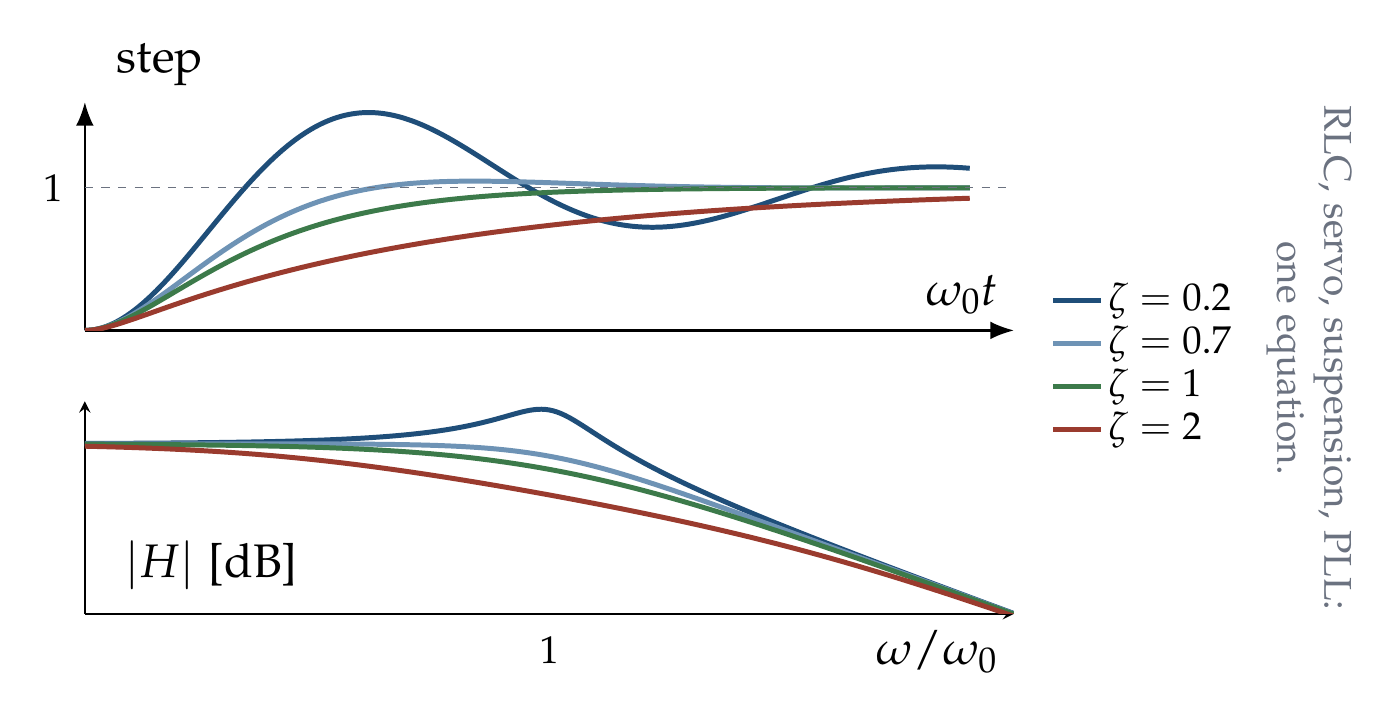
\begin{tikzpicture}
  \begin{axis}[posterplot, name=step, scale only axis, width=118mm, height=29mm, xmin=0, xmax=10.5, ymin=0, ymax=1.6,
     xlabel={$\omega_0 t$}, ylabel={step}, every axis y label/.style={at={(axis description cs:0,1)}, anchor=south west, xshift=2mm},
     xtick=\empty, ytick={1}, samples=140, domain=0:10,
     legend style={draw=none, fill=none, font=\small, at={(1.03,-0.15)}, anchor=west, row sep=-1pt}, legend cell align=left]
    \addplot[accent, smooth] {1-exp(-0.2*x)*(cos(deg(0.9798*x))+0.2041*sin(deg(0.9798*x)))};
    \addlegendentry{$\zeta=0.2$}
    \addplot[accentlt, smooth] {1-exp(-0.7*x)*(cos(deg(0.7141*x))+0.9802*sin(deg(0.7141*x)))};
    \addlegendentry{$\zeta=0.7$}
    \addplot[good, smooth] {1-(1+x)*exp(-x)};
    \addlegendentry{$\zeta=1$}
    \addplot[trap, smooth] {1+(-3.732*exp(-0.268*x)+0.268*exp(-3.732*x))/3.464};
    \addlegendentry{$\zeta=2$}
    \draw[muted, dashed, thin] (axis cs:0,1) -- (axis cs:10.5,1);
  \end{axis}
  \begin{semilogxaxis}[posterplot, name=bode, at={(step.south west)}, anchor=north west, yshift=-9mm, scale only axis, axis lines=left, width=118mm, height=27mm, xmin=0.1, xmax=10, ymin=-40, ymax=10,
     xlabel={$\omega/\omega_0$}, ylabel={$|H|$ [dB]},
     every axis y label/.style={at={(axis description cs:0,0)}, anchor=south west, xshift=3mm, yshift=1mm},
     every axis x label/.style={at={(axis description cs:1,0)}, anchor=north east},
     xtick={1}, xticklabels={$1$}, ytick=\empty, samples=120, domain=0.1:10]
    \addplot[accent, smooth] {-10*log10((1-x^2)^2+(0.4*x)^2)};
    \addplot[accentlt, smooth] {-10*log10((1-x^2)^2+(1.4*x)^2)};
    \addplot[good, smooth] {-10*log10((1-x^2)^2+(2*x)^2)};
    \addplot[trap, smooth] {-10*log10((1-x^2)^2+(4*x)^2)};
  \end{semilogxaxis}
  \node[rotate=-90, anchor=south, text=muted, font=\small, align=center]
    at ($(step.above north east)!0.5!(bode.below south east)+(30mm,0)$) {RLC, servo, suspension, PLL:\\ one equation.};
  \end{tikzpicture}
\end{minipage}

\vspace{6pt}
\trap{Behold, every signal hath two faces, time and frequency: cross over unto the side where the problem is easy, and ye shall find rest. \textbf{Prove all things:} check thy units, thy limits and thy signs; \textbf{hold fast that which is good.}}
\end{tcolorbox}

\vfill
\pair{row1}{c05-state-space}{c06-maxwell}
\vfill
\pair{row2}{c07-power}{c08-noise}
\vfill
\pair{row3}{c09-semiconductors}{c10-logic}
\end{pagecol}
\end{document}
